%%%%%%%%%%%%%%%%%%%%%%%%%%%%%%%%%%%%%%%%%%%%%%%%%%%%%%%%%%%%%%%%%%%%%%%%%%%%%%%%%%%%
% Do not alter this block (unless you're familiar with LaTeX
\documentclass{article}
\usepackage[margin=1in]{geometry} 
\usepackage{amsmath, amsthm, amssymb,amsfonts, fancyhdr, color, comment, graphicx, environ}
\usepackage{xcolor}
\usepackage{mdframed}
\usepackage[shortlabels]{enumitem}
\usepackage{indentfirst}
\usepackage{hyperref}
\usepackage{algorithm2e}
\usepackage{graphicx}
\usepackage{wrapfig}
\usepackage{hyperref}
\usepackage{listings}
\usepackage{subcaption}
\lstset{ 
  language=R,                     % the language of the code
  basicstyle=\normalsize\ttfamily, % the size of the fonts that are used for the code
  numbers=left,                   % where to put the line-numbers
  numberstyle=\normalsize\color{gray},  % the style that is used for the line-numbers
  stepnumber=1,                   % the step between two line-numbers. If it is 1, each line
                                  % will be numbered
  numbersep=5pt,                  % how far the line-numbers are from the code
  backgroundcolor=\color{white},  % choose the background color. You must add \usepackage{color}
  showspaces=false,               % show spaces adding particular underscores
  showstringspaces=false,         % underline spaces within strings
  showtabs=false,                 % show tabs within strings adding particular underscores
  frame=single,                   % adds a frame around the code
  rulecolor=\color{black},        % if not set, the frame-color may be changed on line-breaks within not-black text (e.g. commens (green here))
  tabsize=2,                      % sets default tabsize to 2 spaces
  captionpos=b,                   % sets the caption-position to bottom
  breaklines=true,                % sets automatic line breaking
  breakatwhitespace=false,        % sets if automatic breaks should only happen at whitespace
  keywordstyle=\color{black},      % keyword style
  commentstyle=\color{gray},   % comment style
  stringstyle=\color{teal}      % string literal style
} 
\hypersetup{
    colorlinks=true,
    linkcolor=blue,
    filecolor=magenta,      
    urlcolor=blue,
}


\pagestyle{fancy}


\newenvironment{problem}[2][Problem]
    { \begin{mdframed}[backgroundcolor=gray!20] \textbf{#1 #2} \\}
    {  \end{mdframed}}

% Define solution environment
\newenvironment{solution}
    {\textit{Solution:}}
    {}

\renewcommand{\qed}{\quad\qedsymbol}

% prevent line break in inline mode
\binoppenalty=\maxdimen
\relpenalty=\maxdimen

%%%%%%%%%%%%%%%%%%%%%%%%%%%%%%%%%%%%%%%%%%%%%
%Fill in the appropriate information below
\lhead{Pengju Zhang}
\rhead{CSC-424} 
\chead{\textbf{Assignment 3}}
%%%%%%%%%%%%%%%%%%%%%%%%%%%%%%%%%%%%%%%%%%%%%

\begin{document}
%problem 1
\begin{problem}{1}
\textbf{[10 pts]}
For each of the following datasets, draw the principal component vectors for the dataset, and for their lengths, estimate the size of the eigenvalue (i.e. the variance in the direction of the principal component). Note, you do note need to do this precisely, but you should be able to get a rough estimate from the graph. One question to think about is where should the principal component vectors be based (i.e. where should the arrow’s tail be?)
\end{problem}
\begin{solution}
Note that if two vectors are perpendicular then their dot product equals to 0.
\begin{enumerate}
	\begin{figure}[h]
		\centering
		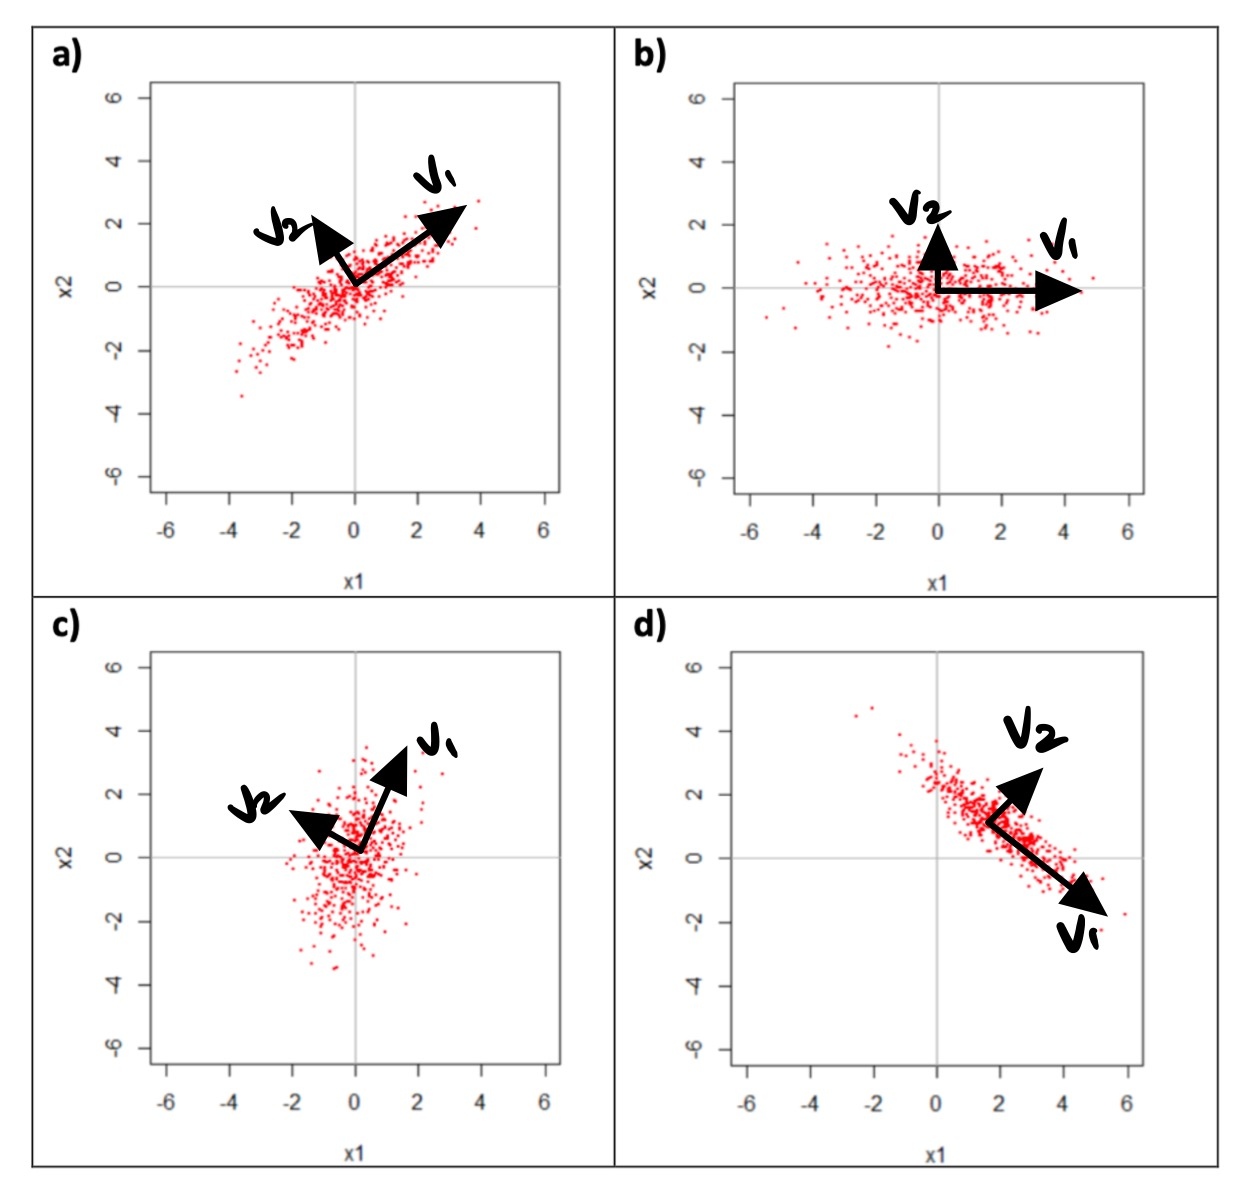
\includegraphics[width=0.7\textwidth]{figure1.jpg}
	\end{figure}
\item \mbox{}
Roughly $v1 = [4, 2]$ and $v2=[-1, 2]$
\item \mbox{}
Roughly $v1 = [4, 0]$ and $v2=[0, 2]$
\item \mbox{}
Roughly $v1 = [4, 2]$ and $v2=[-1, 2]$
\item \mbox{}
Roughly $v1 = [1, -1]$ and $v2=[1, 1]$
\end{enumerate}
\end{solution}

%problem 2
\newpage
\begin{problem}{2}
\textbf{[10 pts]}
Answer each of the following by hand for the following matrices/vectors, and then verify your answers with R code:
\begin{equation}
M = 
\begin{bmatrix}
5 & -1 \\
-1 & 5
\end{bmatrix}, 
N = 
\begin{bmatrix}
21 & -2 & 1 \\
-3 & 10 & -11 \\
3 & -22 & -1
\end{bmatrix},
v =
\begin{bmatrix}
-1\\
1\\
-1
\end{bmatrix}
\end{equation}
\end{problem}
\begin{solution}
\href{run:./src/p2.r}{ (Problem 2 Source Code)}
	\begin{figure}[h]\mbox{}
		\centering
		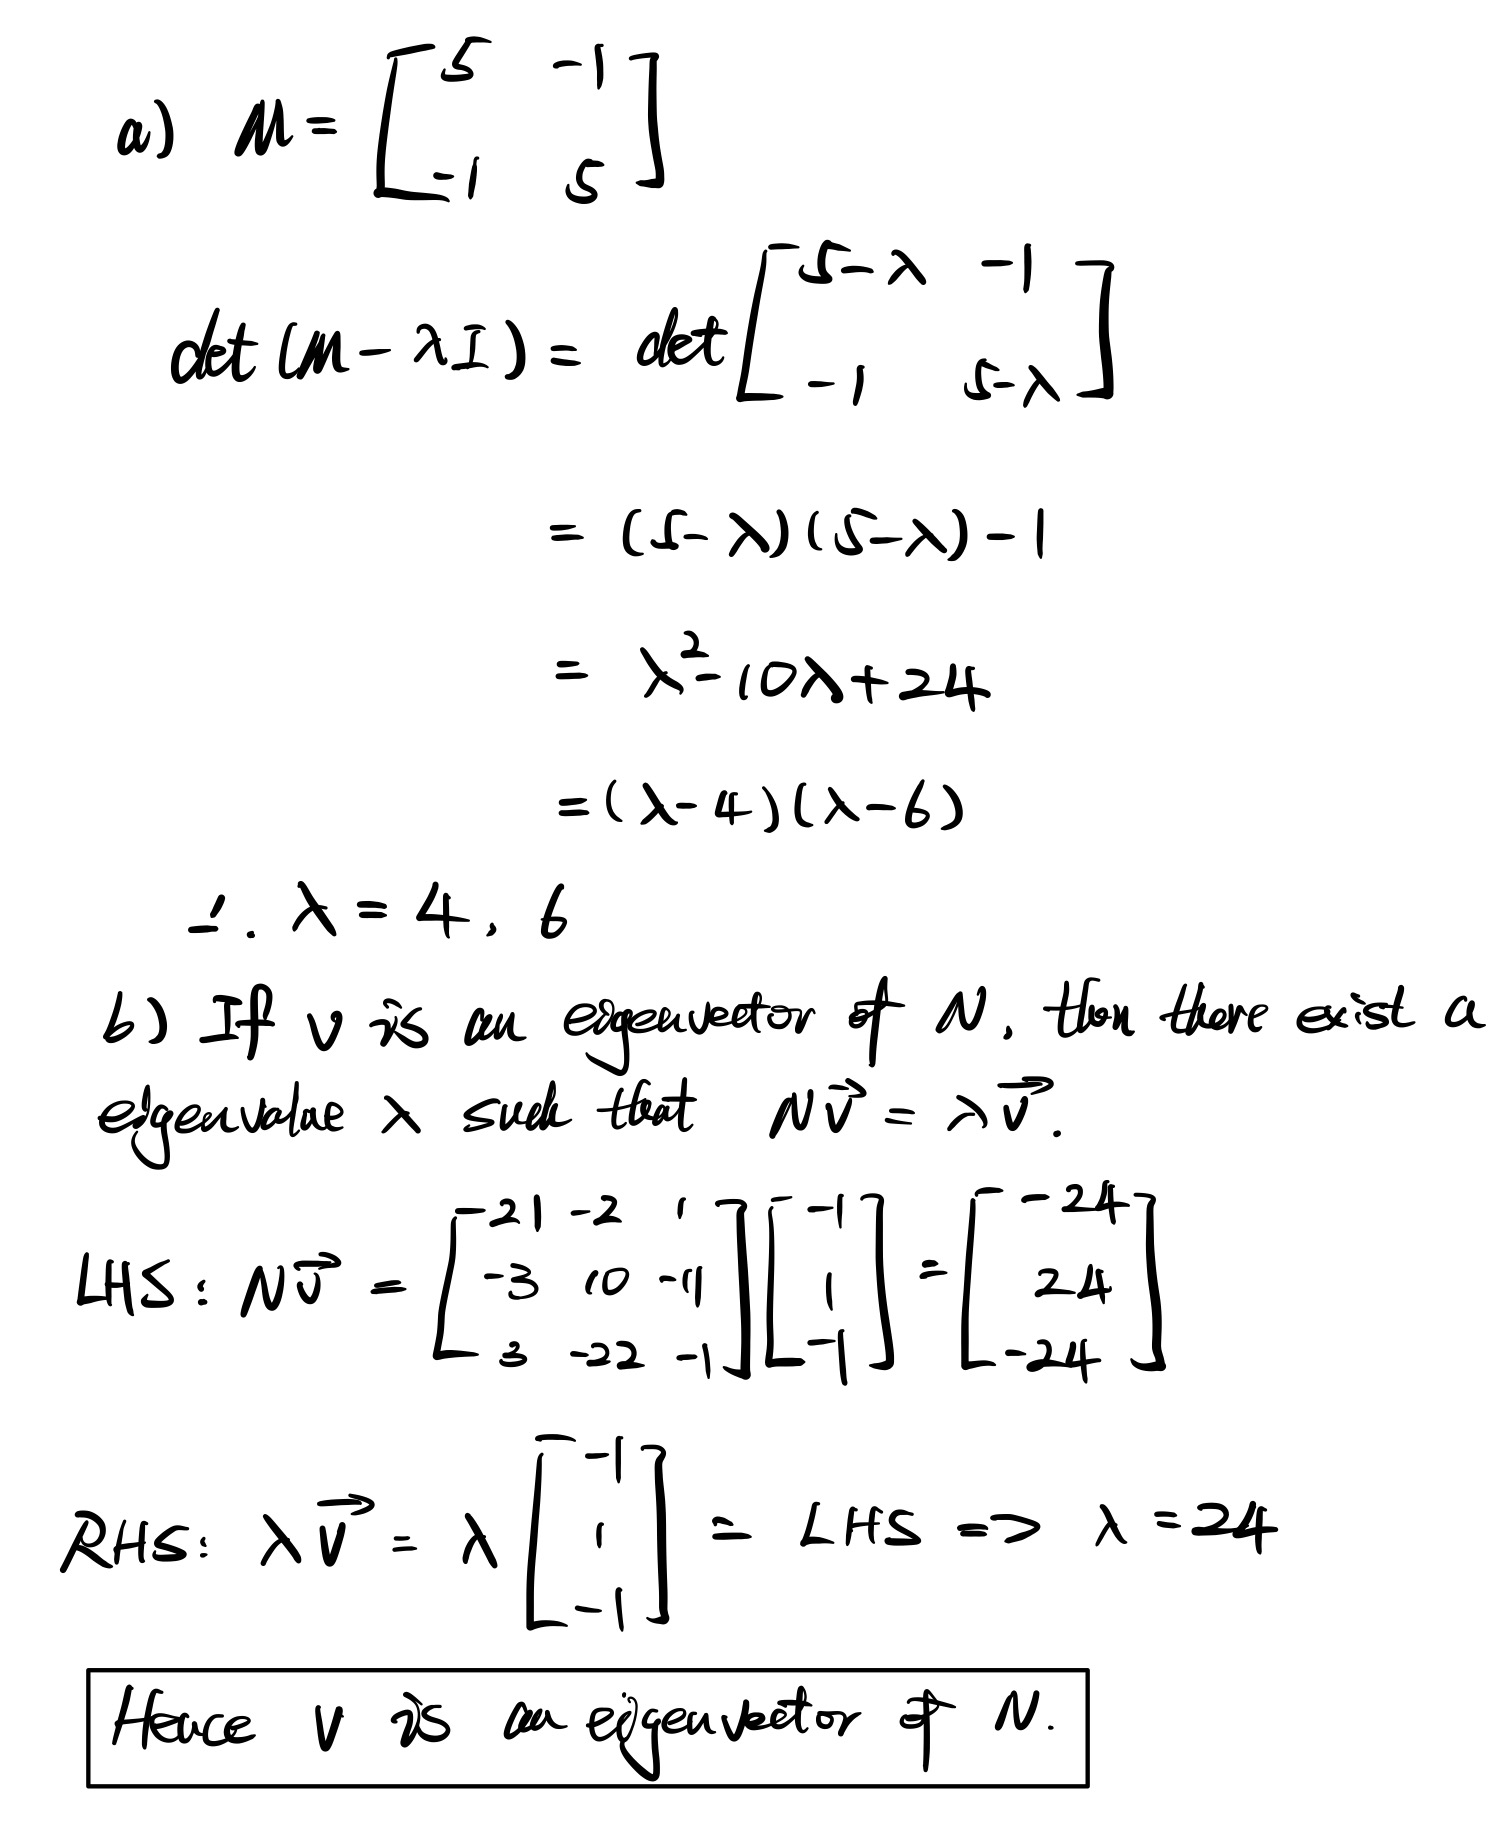
\includegraphics[width=0.8\textwidth]{figure2.jpg}
	\end{figure}
	\newline
c) Eigenvector is 24 for part (b).
\end{solution}

%problem 3
\newpage
\begin{problem}{3}
\textbf{[20 pts]}
Begin with the “census2.csv” datafile, which contains census data on various tracts in a district.
\begin{enumerate}
\item Conduct a principal component analysis using the covariance matrix (the default for prcomp and many routines in other software) and interpret the results. How much of the variance is accounted for in the first component and why is this?
\item Try dividing the MedianHomeValue field by 100,000 so that the median home value in the dataset is measured in \$100,000’s rather than in dollars. How does this change the analysis?
\item Are there any other fields that are in particular need of scaling? Explain why or why not.
\item Compute the PCA with the correlation matrix instead. How does this change the result and how does your answer compare with your answer in b)? How does the meaning of the first component change?
\item Analyze the correlation matrix for this dataset for entries that are significant (i.e. different from zero) at a 95\% confidence level. Are there any variables that are correlated with most of the other variables or are uncorrelated with all of the other variables? What is the importance of doing this and what might you consider doing with such variables?
\item Discuss what using the correlation matrix for PCA does compared to the covariance matrix and why it may or may not be appropriate in this case.
\end{enumerate}
\end{problem}
\begin{solution}
\href{run:./src/p3.r}{ (Problem 3 Source Code)}
\begin{enumerate}
\item\mbox{}
	\begin{lstlisting}
# output
> summary(p)
Importance of components:
                         PC1   PC2   PC3   PC4  PC5
Standard deviation     56447 10.21 6.219 2.247 1.56
Proportion of Variance     1  0.00 0.000 0.000 0.00
Cumulative Proportion      1  1.00 1.000 1.000 1.00
	\end{lstlisting}
The first principal component accounts for 100\% of the variance, and rest of others contain none.
	\begin{lstlisting}
# output
> print(p$rotation)
                        PC1           PC2           PC3           PC4           PC5
Population     8.537905e-07 -4.108282e-02 -7.059713e-02  4.826860e-01  8.719762e-01
Professional   3.775797e-05  7.080539e-02 -7.460074e-02 -8.714029e-01  4.796648e-01
Employed      -1.367095e-06 -5.126328e-01 -8.542663e-01 -1.524163e-02 -8.487872e-02
Government     3.004471e-05  8.546967e-01 -5.095880e-01  8.624903e-02 -4.873218e-02
MedianHomeVal  1.000000e+00 -2.901832e-05  1.701961e-05  2.987813e-05 -1.750755e-05
	\end{lstlisting}
If we step into details in each principal component, we can figure out that MedianHomeVal contributed large proportion of variance in PC1, due to the different scaling factors between MedianHomeVal and all other variables, it lead to MedianHomeVal has over 99.9\% weight among all and result PC1 has 100\% of the variance.
\item\mbox{}
	\begin{lstlisting}
# output
> summary(p2)
Importance of components:
                          PC1    PC2     PC3     PC4     PC5
Standard deviation     10.345 6.2986 2.89324 1.69348 0.39331
Proportion of Variance  0.677 0.2510 0.05295 0.01814 0.00098
Cumulative Proportion   0.677 0.9279 0.98088 0.99902 1.00000
	\end{lstlisting}
By dividing all MedianHomeVal variables by 100,000, the proportion of variance of PC1 becomes 67.7\% which greatly improves the analysis. Since the PCA is much more spread out, we can see by adding PC2, there is a significant increase of cumulative proportion from 67.7\% to 92.79\%.
\item\mbox{}
	\begin{lstlisting}
# output
> head(newData)
  Population Professional Employed Government MedianHomeVal
1       2.67         5.71    69.02       30.3          1.48
2       2.25         4.37    72.98       43.3          1.44
3       3.12        10.27    64.94       32.0          2.11
4       5.14         7.44    71.29       24.5          1.85
5       5.54         9.25    74.94       31.0          2.23
6       5.04         4.84    53.61       48.2          1.60
	\end{lstlisting}
Be aware that Population, Professional, and MedianHomeVal are mostly single digit values, whereas Employed and Government are ten digits, this may introduce a slight bias. However, because these values are percentages unit, it may be best to leave the three percent variables alone, as these differences in values may provide useful information upon further analysis.
\item\mbox{}
	\begin{lstlisting}
# output
> summary(p3)
Importance of components:
                          PC1    PC2    PC3    PC4     PC5
Standard deviation     1.4114 1.1694 0.9296 0.7315 0.49126
Proportion of Variance 0.3984 0.2735 0.1728 0.1070 0.04827
Cumulative Proportion  0.3984 0.6719 0.8447 0.9517 1.00000
	\end{lstlisting}
	\begin{figure}[h]\mbox{}
		\centering
		\begin{subfigure}{.4\textwidth}
  		\centering
  		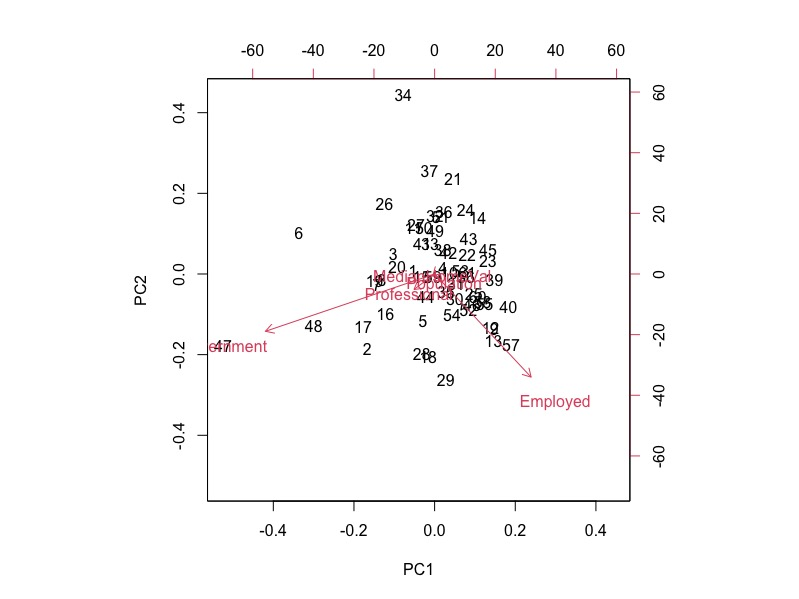
\includegraphics[width=1\linewidth]{Rplot_figure1.jpeg}
  		\caption{Biplot for PCA with Covariance Matrix}
		\end{subfigure}%
		\begin{subfigure}{.4\textwidth}
  		\centering
  		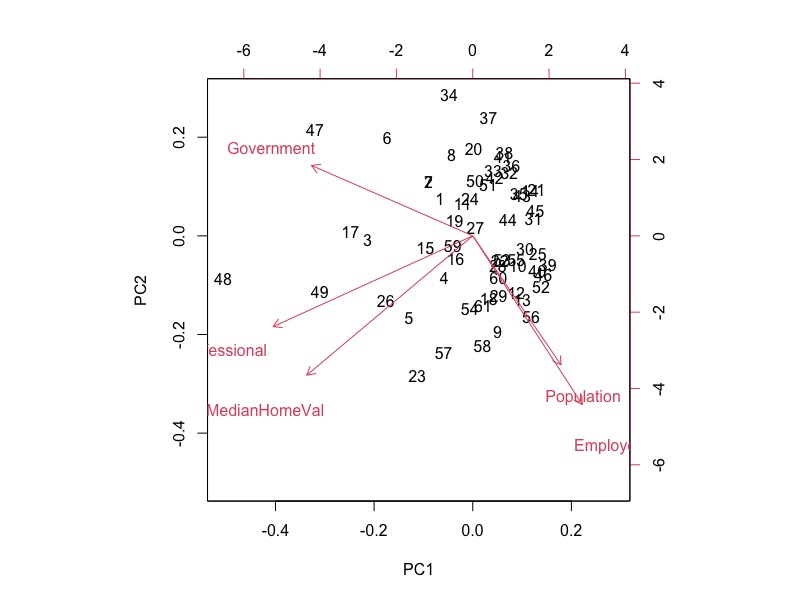
\includegraphics[width=1\linewidth]{Rplot_figure2.jpeg}
  		\caption{Biplot for PCA with Correlation Matrix}
		\end{subfigure}%
	\end{figure}
PCA on correlation is much more informative and reveals some structure in the data and relationships between variables. But standardizing each of the variables will leave them equal weight, note that the explained variances for PC1 drop to 39.84\% due to the less impact on the main variables.
\item\mbox{}
	\begin{lstlisting}
# output
> corrTest = corr.test(newData, adjust="none")
> x = corrTest$p
> xTest = ifelse(x<0.05, T, F)
> xTest
              Population Professional Employed Government MedianHomeVal
Population          TRUE        FALSE     TRUE      FALSE         FALSE
Professional       FALSE         TRUE    FALSE       TRUE          TRUE
Employed            TRUE        FALSE     TRUE       TRUE         FALSE
Government         FALSE         TRUE     TRUE       TRUE         FALSE
MedianHomeVal      FALSE         TRUE    FALSE      FALSE          TRUE
	\end{lstlisting}
The only significant relationship was between professional and medianHomeValue. This makes sense because we would expect someone with higher education to have a higher income, as a result, a higher median value home.
\item\mbox{}
You tend to use the covariance matrix when the variable scales are similar and the correlation matrix when variables are on different scales. Using the correlation matrix is equivalent to standardizing each of the variables (to mean 0 and standard deviation 1). In general, PCA with and without standardizing will give different results. Especially when the scales are different.
\end{enumerate}
\end{solution}
%problem 4
\newpage
\begin{problem}{4}
\textbf{[20 pts]}
The data given in the file ‘Employment.txt’ is the percentage employed in different industries in Europe countries during 1979. Techniques such as Principal Component Analysis (PCA) can be used to examine which countries have similar employment patterns. 
\begin{enumerate}
\item Is scaling appropriate for this data? Explain why or why not.
\item Note that whatever your answer for c) the “principal” function will scale your data. This is because scaling is the default behavior in factor analysis. So, compute an initial principal component analysis using “prcomp” with scaling and apply the knee and var=1 criteria. How many components does each method suggest? Explain how confident you are in this result and if there are any ambiguities, why you made the choice you did.
\item Is VARIMAX factor rotation being applied in your computation in b)? Explain.
\item Print the component coefficients for the number of components you chose in b). For each component, write out the formula and give a brief interpretation. How easy are they to separate in-terms of meaning?
\item Run a parallel analysis for this dataset to compute a suggested number of components. Use the results of this and what you got with the knee and var=1 to choose a number of components. Explain your choice in detail.
\item Use “principal” to compute the Principal Factor Analysis with this number of components, and with VARIMAX factor rotation. Give the formula for each component and a brief interpretation. Has rotating improved the ability to interpret the components?
\item What countries have the highest and lowest values for each factor (only include the number of components specified in part e). For each of those countries, give the principal component scores (again only for the number of components specified in part a).
\item Consider the loadings matrix in e, how appropriate is the number of components you selected? Try running the analysis with one more and one fewer component. What do the results suggest for the number of components to finally select?
\end{enumerate}
\end{problem}
\begin{solution}
\href{run:./src/p4.r}{ (Problem 4 Source Code)}
\begin{enumerate}
	\begin{figure}[h]\mbox{}
		\centering
		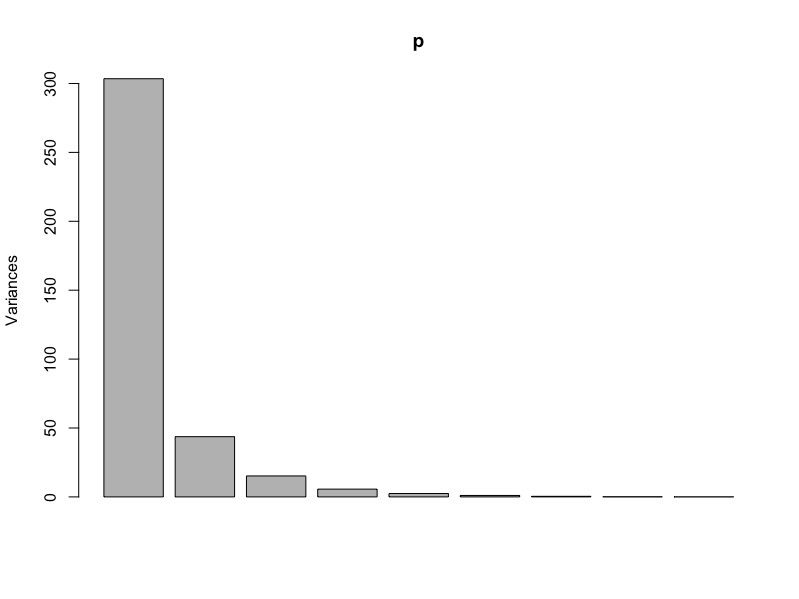
\includegraphics[width=0.8\textwidth]{Rplot_figure4.jpeg}
		\caption{PCA screeplot}
	\end{figure}
	\newpage
\item This might need scaling. Looking at the output from our prcomp() command we see moving left to right that by the second component we already have a cumulative proportion of 93.33\% the variability.
\newpage
\item 
	\begin{lstlisting}
# output
> summary(p)
Importance of components:
                          PC1    PC2    PC3    PC4     PC5    PC6     PC7    PC8      PC9
Standard deviation     1.8674 1.4595 1.0483 0.9972 0.73703 0.6192 0.47514 0.3699 0.006755
Proportion of Variance 0.3875 0.2367 0.1221 0.1105 0.06036 0.0426 0.02508 0.0152 0.000010
Cumulative Proportion  0.3875 0.6241 0.7462 0.8568 0.91711 0.9597 0.98480 1.0000 1.000000
	\end{lstlisting}
	\begin{figure}[h]\mbox{}
		\centering
		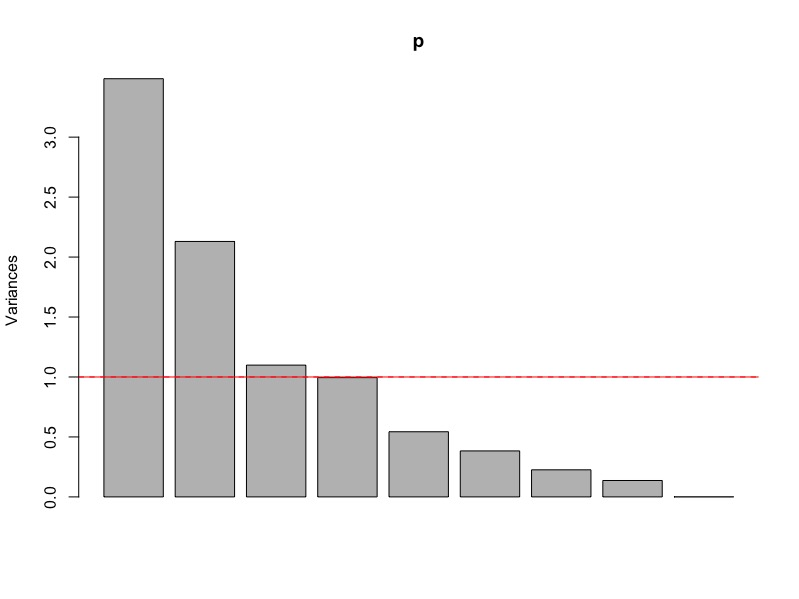
\includegraphics[width=0.8\textwidth]{Rplot_figure3.jpeg}
		\caption{PCA screeplot}
	\end{figure}
Clearly we can see that there are four components $\geq$ line at 1.0, by adding the first four largest variance we have 0.8568 proportion. We’ll end up with 4 vectors reducing the dimensionality of our data while minimizing loss and accounting for 85.68\% of the variance within our original dataset.
\item
\newpage
\item
	\begin{lstlisting}
# output
> p$rotation
             PC1         PC2         PC3         PC4        PC5        PC6         PC7          PC8        PC9
Agr  0.523790989  0.05359389  0.04867439 -0.02879285  0.2127026  0.1533066  0.02132116  0.007922069 0.80641788
Min  0.001323458  0.61780714 -0.20110021 -0.06408495 -0.1637431 -0.1005897 -0.72571894  0.088362816 0.04856307
Man -0.347495131  0.35505360 -0.15046308  0.34608821 -0.3849576 -0.2881523  0.47936298  0.125818308 0.36595728
PS  -0.255716182  0.26109606 -0.56108325 -0.39330897  0.2951715  0.3572641  0.25564699 -0.341228167 0.01938500
Con -0.325179319  0.05128845  0.15332114  0.66832395  0.4715934  0.1303542 -0.22069499 -0.355733906 0.08257219
SI  -0.378919663 -0.35017206 -0.11509551  0.05015651 -0.2835681  0.6148287 -0.22943536  0.387536806 0.23829861
Fin -0.074373583 -0.45369785 -0.58736130  0.05156652  0.2795682 -0.5255581 -0.18745525  0.174329338 0.14517064
SPS -0.387408806 -0.22152120  0.31190350 -0.41223019 -0.2203514 -0.2629097 -0.19130212 -0.506154178 0.35094226
TC  -0.366822713  0.20259185  0.37510601 -0.31437188  0.5129356 -0.1239760  0.06819331  0.544562381 0.07205520
	\end{lstlisting}
	
\end{enumerate}
\end{solution}
%problem 5
\newpage
\begin{problem}{5}
\textbf{[20 pts]}
For this problem, you will analyze partial from intelligence tests given to children. Each child was given 11 tests on which they were rated.
\begin{enumerate}
\item Should the data be scaled or not for running PCA? Explain why/why not in detail.
\item Run an initial corrplot and an initial unrotated PCA (i.e. no VARIMAX). Use the corrplot and the techniques from the lecture to determine the appropriate number of factors to
extract. Are there any variables that will likely be single-variable factors? Explain.
\item Run a Principal Factor Analysis with VARIMAX rotation and report the loadings with a
cutoff of .4, and also plot the contributions to the components using either a biplot or PCA\_Plot\_Psych. Analyze the loadings and the plot. How clean and useful are the variable separations? Give a name to each component.
\item Then sort the scores by the first and second component (you will have to do this separately for each). Consider the cases (children) that score highly or extremely low on each. What do the scores mean for each of these cases? Are there any surprises?
\item Run a Common Factor Analysis (exploratory) and compare the loadings to those of the principal factor analysis. Note any significant differences and explain how they affect the factors practically.
\end{enumerate}
\end{problem}
\begin{solution}
\href{run:./src/p5.r}{ (Problem 5 Source Code)}
\begin{enumerate}
\item No scaling is needed because all the variables measure in similar range and we can assume that the grading method was not changed from test to test as this would make little practical since when comparing performance across the factors.
\item\mbox{}
	\begin{figure}[h]\mbox{}
		\centering
		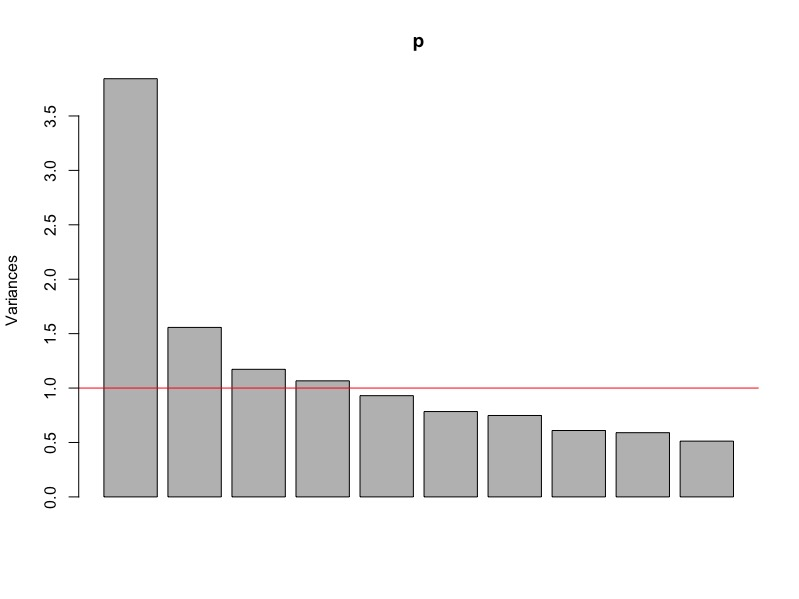
\includegraphics[width=0.8\textwidth]{Rplot_figure5.jpeg}
		\caption{PCA screeplot}
	\end{figure}
	\begin{lstlisting}
# output
> summary(p)
Importance of components:
                          PC1    PC2     PC3     PC4     PC5     PC6     PC7     PC8     PC9    PC10    PC11    PC12    PC13
Standard deviation     1.9602 1.2479 1.08268 1.03260 0.96434 0.88552 0.86487 0.78101 0.76805 0.71582 0.68415 0.63896 0.55805
Proportion of Variance 0.2955 0.1198 0.09017 0.08202 0.07154 0.06032 0.05754 0.04692 0.04538 0.03941 0.03601 0.03141 0.02396
Cumulative Proportion  0.2955 0.4153 0.50551 0.58753 0.65906 0.71938 0.77692 0.82384 0.86922 0.90863 0.94464 0.97604 1.00000
	\end{lstlisting}
\item\mbox{}
	\begin{figure}[h]\mbox{}
		\centering
		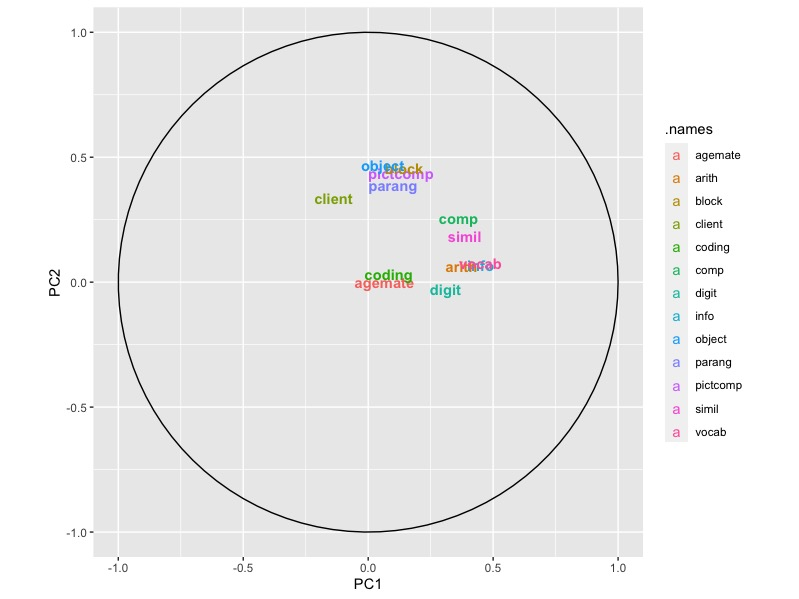
\includegraphics[width=0.8\textwidth]{Rplot_figure6.jpeg}
		\caption{PCA Plot}
	\end{figure}
	\begin{lstlisting}
# output
Loadings:
         RC1    RC2    RC3   
client           0.502       
agemate                -0.444
info      0.802              
comp      0.644              
arith     0.665              
simil     0.688              
vocab     0.801              
digit     0.551              
pictcomp         0.647       
parang           0.578       
block            0.678       
object           0.697       
coding                  0.819

                 RC1   RC2   RC3
SS loadings    3.177 2.207 1.187
Proportion Var 0.244 0.170 0.091
Cumulative Var 0.244 0.414 0.506
	\end{lstlisting}
\item\mbox{}
After sorting the components, we see that RC1 has extreme negative values of -2.47, indicating that the individual performed very poorly on all of the intelligence tests, whereas the high scores of 3.06 indicate that the individual performed very well on all of the tests. The extreme values of the RC2 show a minimum of -3.77, indicating very poor performance on the more spatial and visual intelligence tests, while values in the 2.5-1.5 range represent good performance on the pictorial intelligence tests.
\item\mbox{}
	\begin{lstlisting}
# output
Loadings:
         Factor1 Factor2 Factor3
info      0.632           0.463 
comp      0.574                 
simil     0.560                 
vocab     0.763                 
pictcomp          0.587         
block             0.582         
object            0.587         
arith                     0.536 
client                          
agemate                         
digit                           
parang            0.466   0.410 
coding                          

               Factor1 Factor2 Factor3
SS loadings      2.007   1.612   1.070
Proportion Var   0.154   0.124   0.082
Cumulative Var   0.154   0.278   0.361
	\end{lstlisting}
The loadings on Factors 1, 2, and 3 are generally lower than in the principal factor analysis. Except for factor 3, this optimized method for computing the factors appears to be in agreement with the principal factor method. While both factors have coding contributions, indicating that it may be a separate group that should be included, the models disagree on what other variables are related to it. Another thing it could be telling us is that it is not necessary and may even be preferable to include only two factors, one for overall performance and the other for differences in spatial intelligence.
\end{enumerate}
\end{solution}


%problem 6
\newpage
\begin{problem}{6}
\textbf{[Paper Review]}
\end{problem}
\begin{solution}
\begin{enumerate}
\item They are using PCA to try to understand the underlying variables and why gene responses vary under different conditions. As a result, they are attempting to deduce the interpretations from the underlying variables. Since this type of dataset is prone to vague correlations that are difficult to trace, they are also looking to reduce the noise that is often associated with such experiments.
\item Instead of scaling the data and employing the correlation matrix, they chose to perform natural log transformations on gene expression ratios to mitigate the impact of any gene on the rest of the data. They do not equalize the variance to 1 for similar reasons.
\item They do rotate the factors to align them with the principal component axes. They use orthogonal rotation to align the data with the axes of the principal components so that they can measure it against the direction of greatest variance.
\item They can capture 90 percent of the variability with just the first two components, by adding three components increases to 95 percent. They used a single criterion to determine how many components to include, discarding all components that accounted for less than (70/n) percent of the overall variability.
\item They do not appear to discuss the components' stability or how the components might change in the presence of a different sample. Additional research should be conducted to either disprove or demonstrate this issue.
\item Using PCA and being able to find a condense set of variables to discover useful insights into their data. Despite the fact that there were seven experiments in the times series, each gene had only two or three features. They were able to determine which variables contributed to the gene's overall expression, changes in expression over time, and concavity while reducing the complexity of their interpretations.
\end{enumerate}
\end{solution}
\end{document}